%%%%%%%%%%%%%%%%%%%%%%%%%%%%%%%%%%%%%%%%%%%%%%%%%
%%%%%%%%%%%% cap: intro %%%%%%%%%%%%%%%%%
%%%%%%%%%%%%%%%%%%%%%%%%%%%%%%%%%%%%%%%%%%%%%%%%%

\chapter{Introduction}\label{cap:intro}

DataManager is designed with the users' phones' data management in the foreground, focusing on a simple interface that doesn't require much from the user, with options for emptying their trash, cleaning unneeded data, and being able to see what applications they have not used regularly, each done with one press of a button only.

The app offers different menus for each of its use cases, each with an easy-to-use and easy-to-understand layout. For further convenience, the app also offers the ability to enter a general settings menu where the user can change the overall theme of the app, from a light theme to a dark one, and to change the language from English to Romanian.

The three main screens of the app consist of the cache cleaning screen, the unused applications screen, and the main menu screen. The main menu gives access to the other screens, the option to empty the trash folder, and the general settings screen, where the user can change certain preferences about the application. The other two screens are for data management, the cache screen allows the user to select filters for what he wants to delete, and the unused applications screen lists the applications of the user and the last time they were used, with the option to delete them if he wished to.

For accessing the storage, internet, and so on, the application will ask the user for the required permissions. All permissions are described in a special menu found in the main menu that tells the user exactly what are they used for.

\newpage

\section{Motivation}\label{sect:Motivation}

\begin{wrapfigure}{r}{0.4\textwidth} 
    \centering
    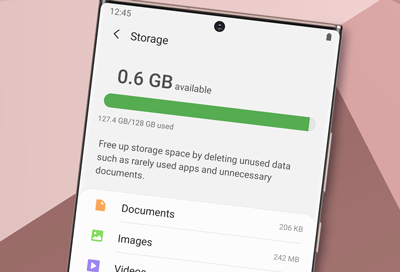
\includegraphics[width=0.4\textwidth]{storage.png}
    \caption{The common sight of an emptying storage}
    \label{fig:batteryImage}
\end{wrapfigure}

Owning a phone has become in the last decade a basic human need for all of us, regardless of age, culture, or background. The phone helps connect us with one another, not just by making phone calls or writing messages to one another, but modern phones also allow us to use the internet, share our stories, photos, life experiences, and so much more. Besides connecting with one another, it gives us countless possibilities, from entertaining us to educating us and so on. 

Owning to this fact, one of the most important factors of our phones, that we usually do not take into consideration or notice too late is the well-being of the phone, usually being represented by the neglect of our storage spaces. It is easy to lose track of our storage and find ourselves in the awkward situation of needing to take a picture, download a file for work, or just install the hottest new app, and being unable to do so because we are hit with the surprise of no more storage space left. Not only that, but one aspect of the phone that everybody seems to not pay attention to is the well-being of the phone, many forget to delete leftover data from uninstalled applications, empty the trash folder, and so on, little things that in time add up to a worse functioning phone and a smaller storage space.

Such unneeded files like caches, logs, \ac{APK} files, and so on, are the type of files that the user will never think about, and especially not think to clean up to save on his or her phone memory.

\section{Problem Statement}\label{sect:Problem Statement}

This problem becomes more and more prevalent with the size of newer applications, the increase in resolution for photos and videos, and the amount of data that remains from them. A simple 1080\ac{p} photo is around 6 \ac{MB}, while a phone with \ac{4K} capabilities is around 24 \ac{MB}, which is an increase of 4 times. Things are even worse when looking at video memory, a 1080\ac{p} 1-minute video has around 100 \ac{MB} while a \ac{4K} one has around 450 \ac{MB}.

With this in mind, every little amount of memory that the user can save up is usually more than welcomed, but unfortunately, phones do not come with built-in memory managers from the manufacturers.

As such, the problem of how to save our storage space for our phones usually remains in the hands of the consumer, usually by downloading a third-party application that gets the job done. 
\newpage

\section{Thesis Scope and Objectives}\label{sect:Thesis Scope and Objectives}

Possible solutions to such problems include the very functions of the proposed application, with how much we tend to use our phones in everyday life, too little time is spent taking care of them and managing their storage in a healthy manner.

The improvements will have certain liberties that the user will have to give his consent to, such as the functionality to access the external storage and usage for the application, however, such improvements will prove fruitful to those who want an increase in storage space, without the need for searching through every application for signs of residual data.

\section{Thesis Structure}\label{sect:Thesis Structure}

The thesis will have a format consisting of 5 main chapters, each with various sections, each chapter looking at a different aspect of the thesis. The 5 chapters are as follows:

    • The first chapter focuses on the what and the why of the project, sharing the motivation behind the project and a general overview behind it;

    • The second chapter looks at the application architecture, its main use cases, its main flow, and the expected app requirements;

    • Chapter 3 focuses on similar applications that are in the same genre as this thesis, looking at their varied utilities, and functions, and concluding at the end of the chapter with a comparison between them;

    • Chapter 4  looks at the implementation that was used for creating the application, and the methods and classes that were used;

    • The last chapter is the user manual for the application, guiding the user through each of the main screens, what they do, what permissions they require, and what setting options the user has access to;

After these chapters, the app will also have a chapter for conclusions and discussions based on the results, as well as a bibliography for users' reference.